%!TEX root = ../main.tex

\chapter{Abläufe}
\label{ch:processes}

Im folgenden Kapitel werden die wichtigsten Abläufe des Systems beschrieben und zur Veranschaulichung in
Diagrammen dargestellt.

\section{Anmeldeprozess}

Das Programm ist so aufgebaut, dass man sich für die Interaktion mit dem System zuerst anmelden muss.
Man kann sich als Administrator*in, als Gast oder mit dem KIT-Account anmelden.

Hier wird der Ablauf des Anmeldens in einem Diagramm beschrieben.

\begin{figure}[ht]
    \centering
    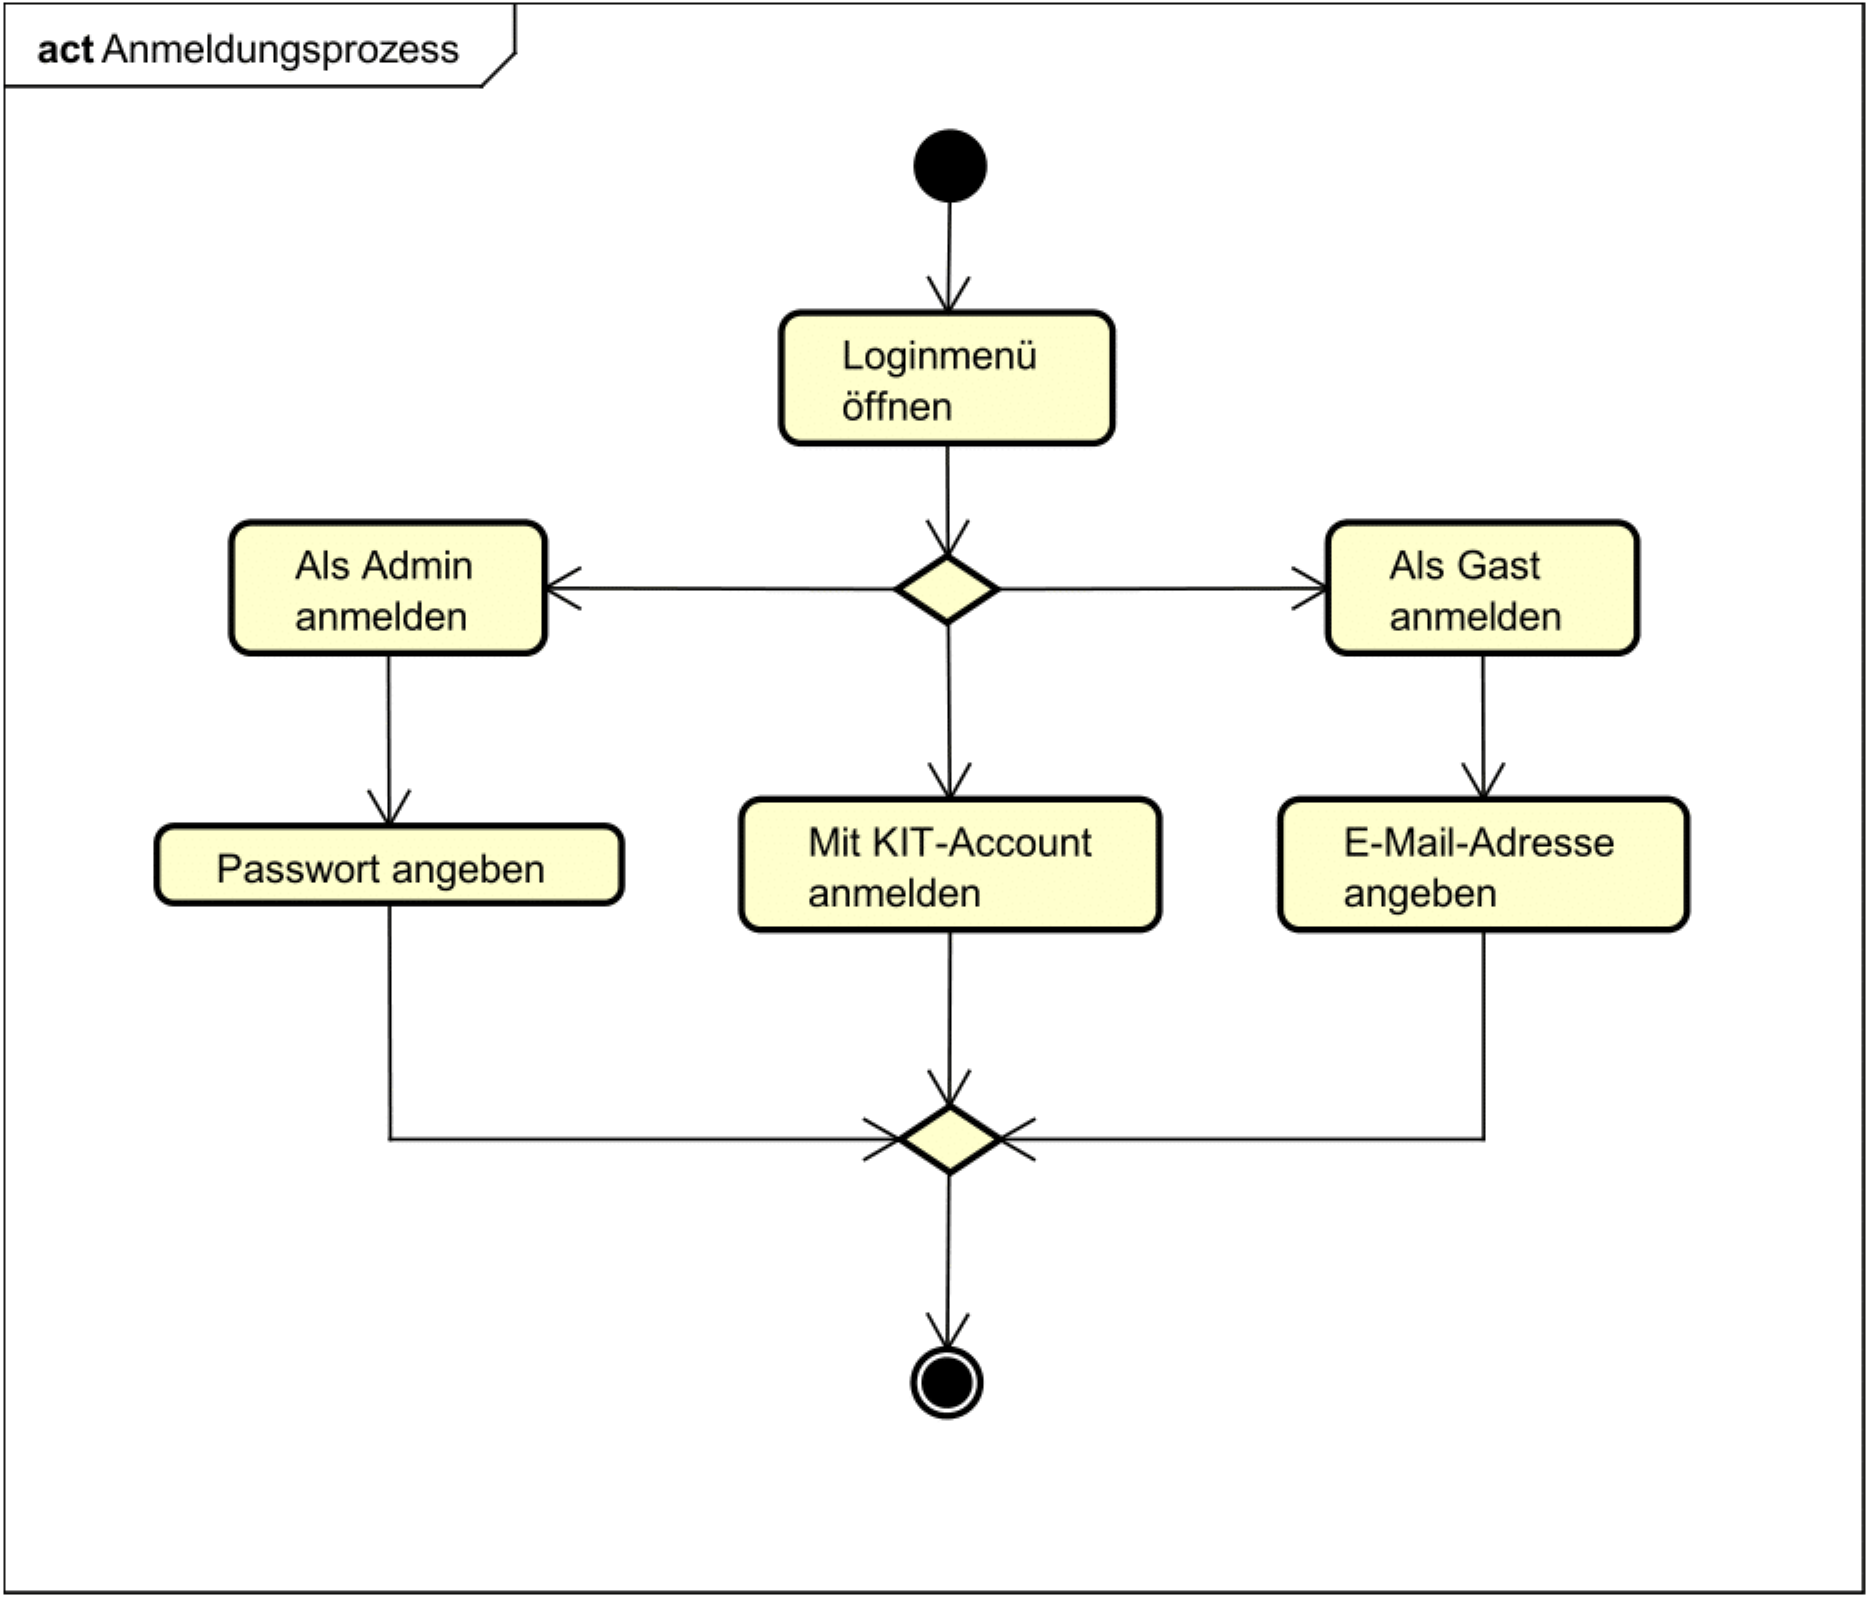
\includegraphics[width=\textwidth]{figures/activity/anmeldeprozess}
    \caption{Diagramm zur Erklärung des Anmeldeprozesses}
    \label{fig:login-diagram}
\end{figure}
\clearpage

\section{Buchung Erstellen}

\subsection{Nutzer*in erstellt Buchung}

 Weiterhin können Buchungen erstellt werden. Mit der Voraussetzung, dass die nutzende Person angemeldet ist,
kann die Buchungsansicht geöffnet werden. Dann gibt muss eine Priorität angegeben werden und festgelegt werden,
 ob man den Raum teilen möchte. Hier sind die Auswahlmöglichkeiten "Ja", "Nein" und "Auf Anfrage". Bei den "Auf
 Anfrage" gestellten Buchungen können Nuter*innen über die Website Anfragen stellen, wenn sie den Termin mit nutzen
 wollen. Weiterhin kann der ausgewählte Zeitraum angepasst oder eine Beschreibung angegeben werden.

 Das Ablaufdiagramm beschreibt den Ablauf einer Terminerstellung.

\begin{figure}[ht]
    \centering
    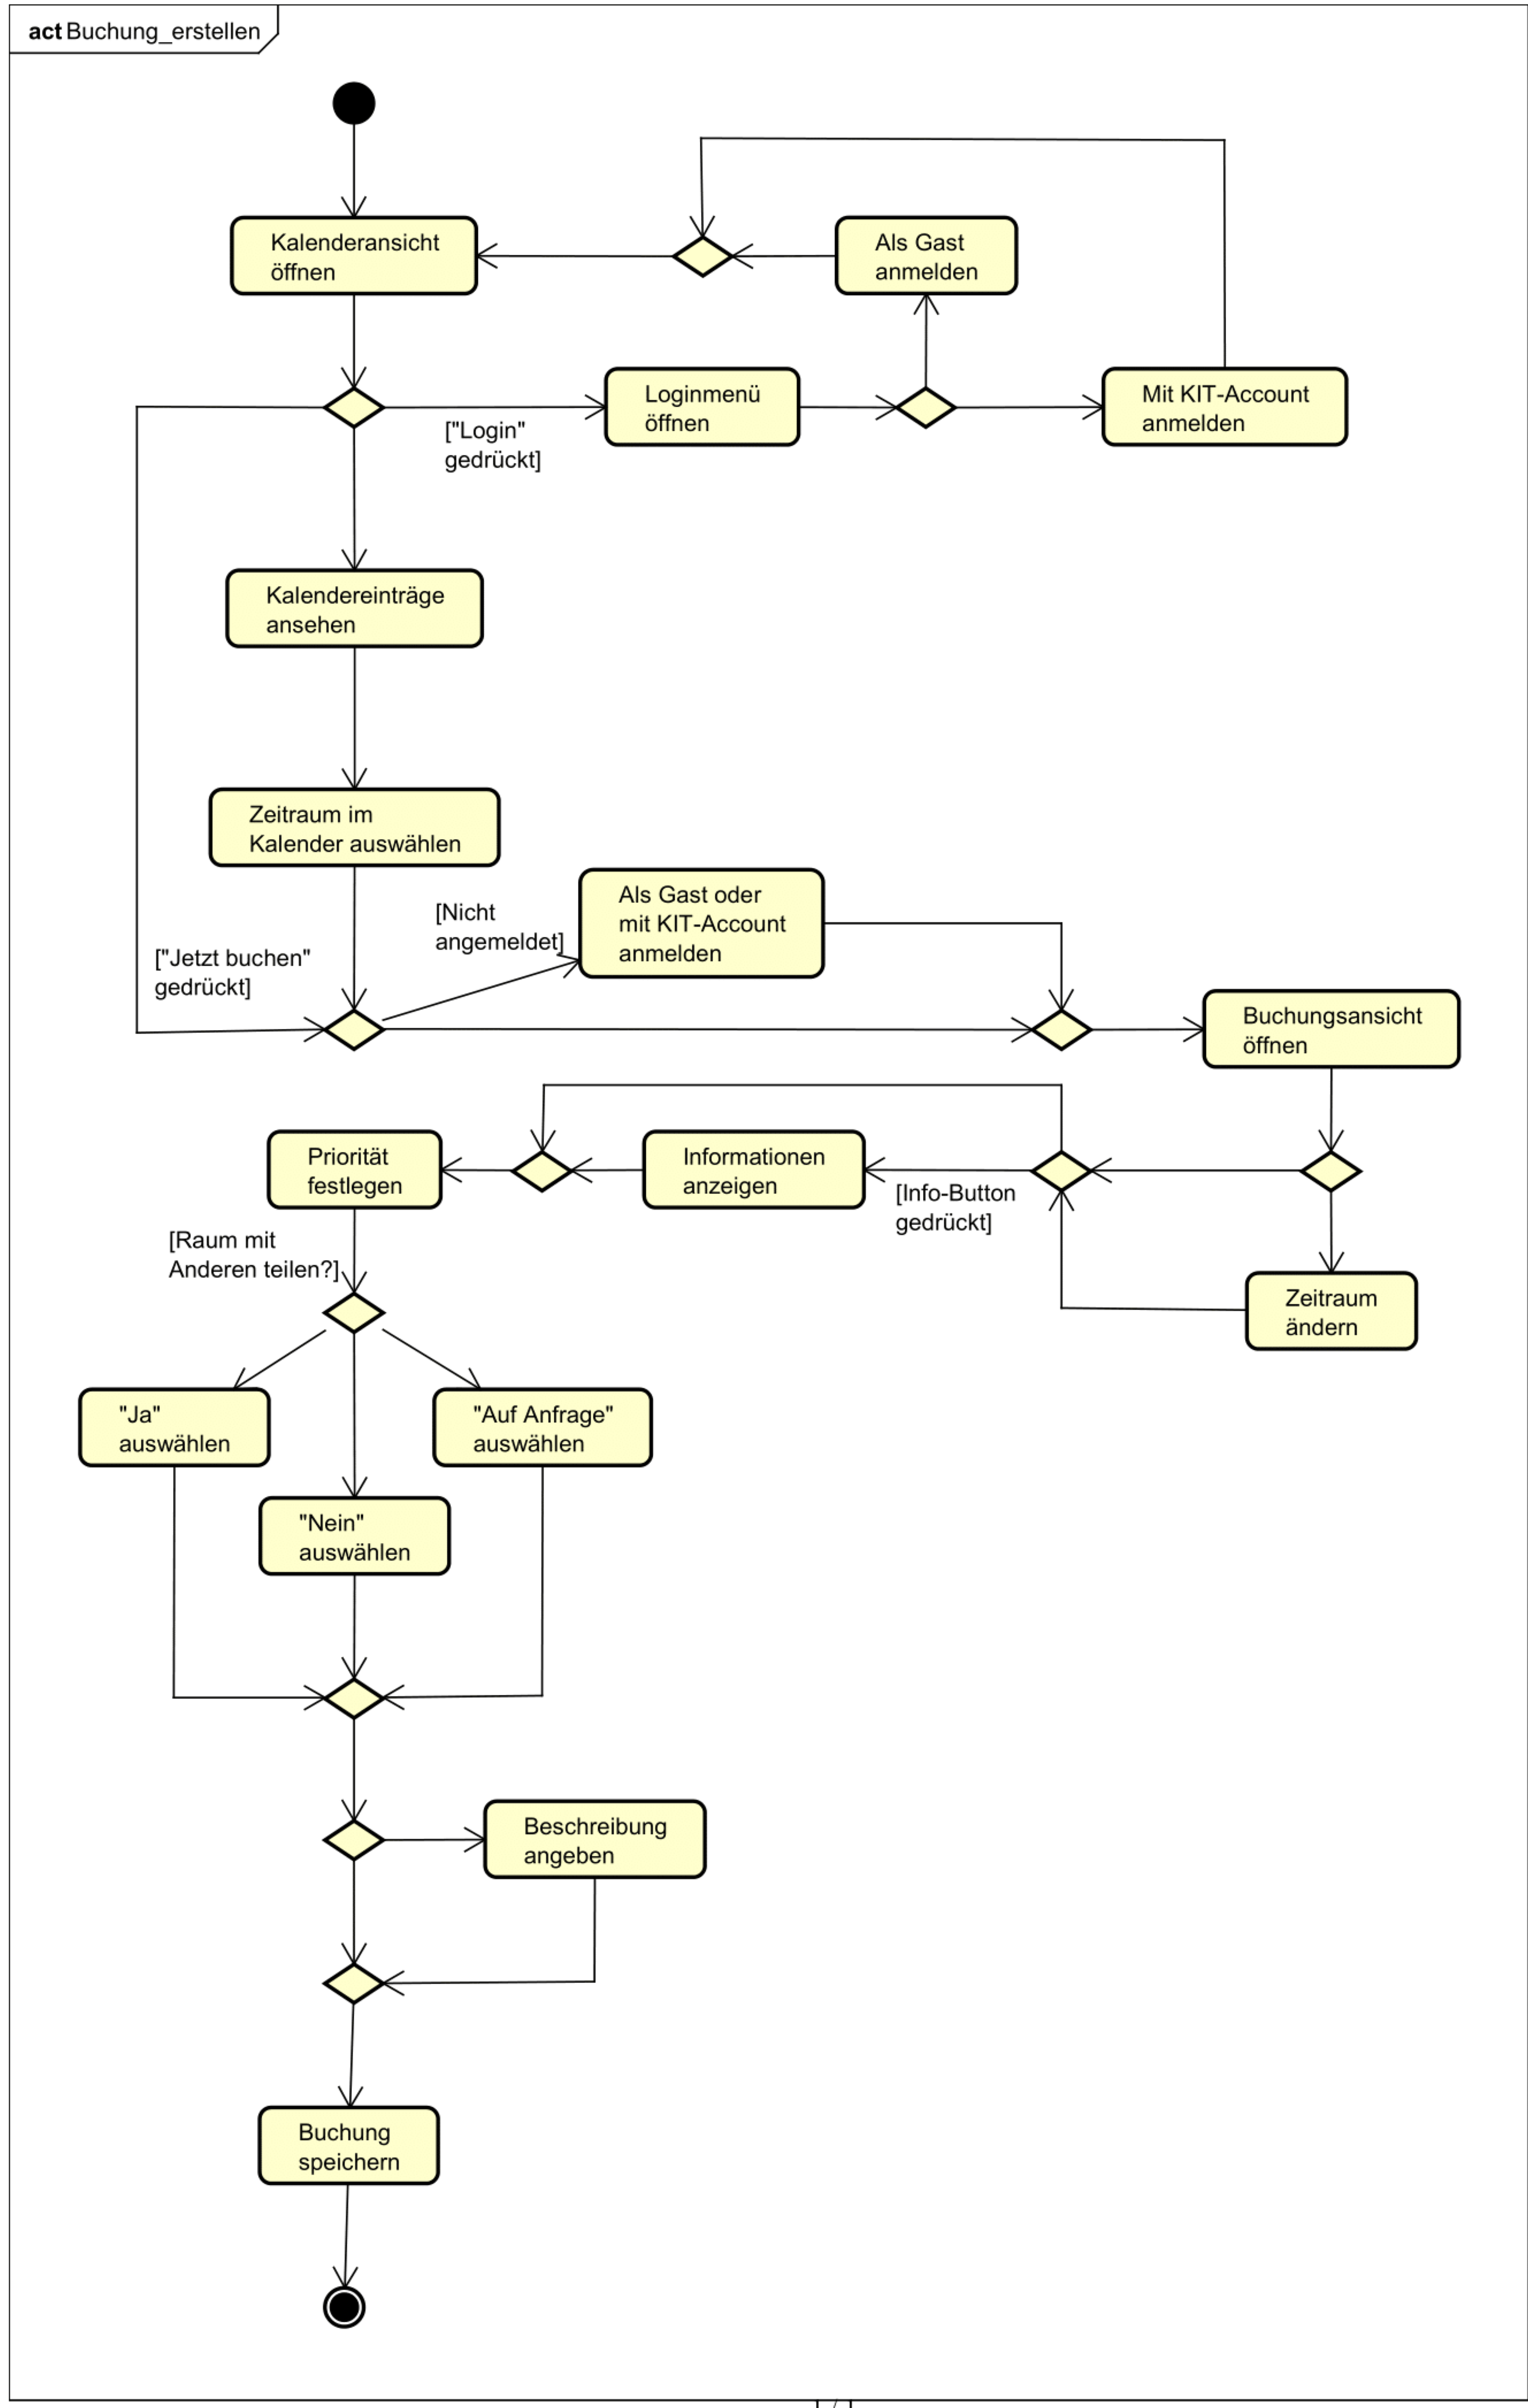
\includegraphics[width=\textwidth]{figures/activity/buchungerstellen}
    \caption{Diagramm zur Erklärung des Buchungserstellungsprozesses}
    \label{fig:make-booking-diagram}
\end{figure}

\subsection{Konfliktlösung bei Buchungserstellung}

Bei der Erstellung eines Termins kann ein Terminkonflikt auftreten, falls im angegebenen Zeitraum bereits eine
Buchung getätigt wurde. In diesem Fall wird nach der Priorität der Buchung entschieden und die Buchung mit
höherer Priorität wird beibehalten. Im Fall, dass beide Buchungen die gleiche Priorität haben, wird die zuerst
erstellte Buchung beibehalten. Wenn beide Buchungen bei der Kategorie "Raum teilen" auf "Ja" gesetzt sind, wird die
Buchung mit der niedrigeren Priorität beibehalten. Falls die zuerst getätigte Buchunge auf "Auf Anfrage" steht,
besteht die Möglichkeit eine Anfrage zu stellen.

Das Ablaufdiagramm stellt den oben beschrieben Konliktlösungsprozess dar.

\begin{figure}[ht]
    \centering
    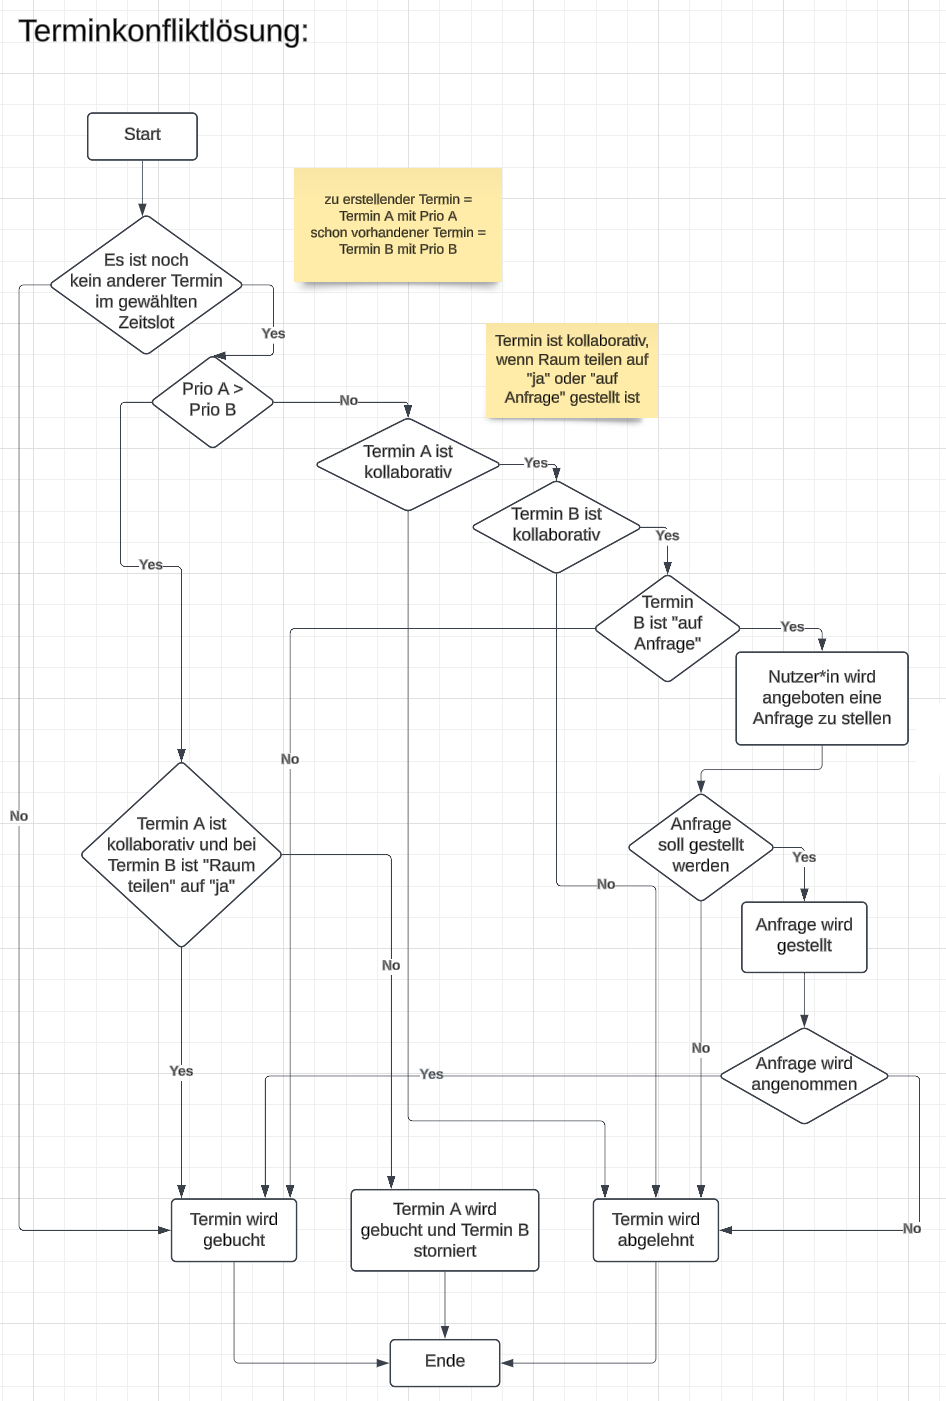
\includegraphics[width=\textwidth]{figures/activity/terminkonfliktloesung}
    \caption{Diagramm zur Erklärung des Konfliktlösungsprozesses bei der Buchungserstellung}
    \label{fig:resolve-conflict-diagram}
\end{figure}
\clearpage

\section{Buchungen Verwalten}

Die Website bietet die Möglichkeit, die eigenen Buchungen zu verwalten. Mit der Voraussetzung,
dass man angemeldet ist, kann man die Terminübersicht, welche eine Liste der eigenen Termine anzeigt,
öffnen und hat dann die Möglichkeit Termine zu löschen.

Das Ablaufdiagramm beschreibt den Ablauf des Buchungsverwaltungsprozesses.

\begin{figure}[ht]
    \centering
    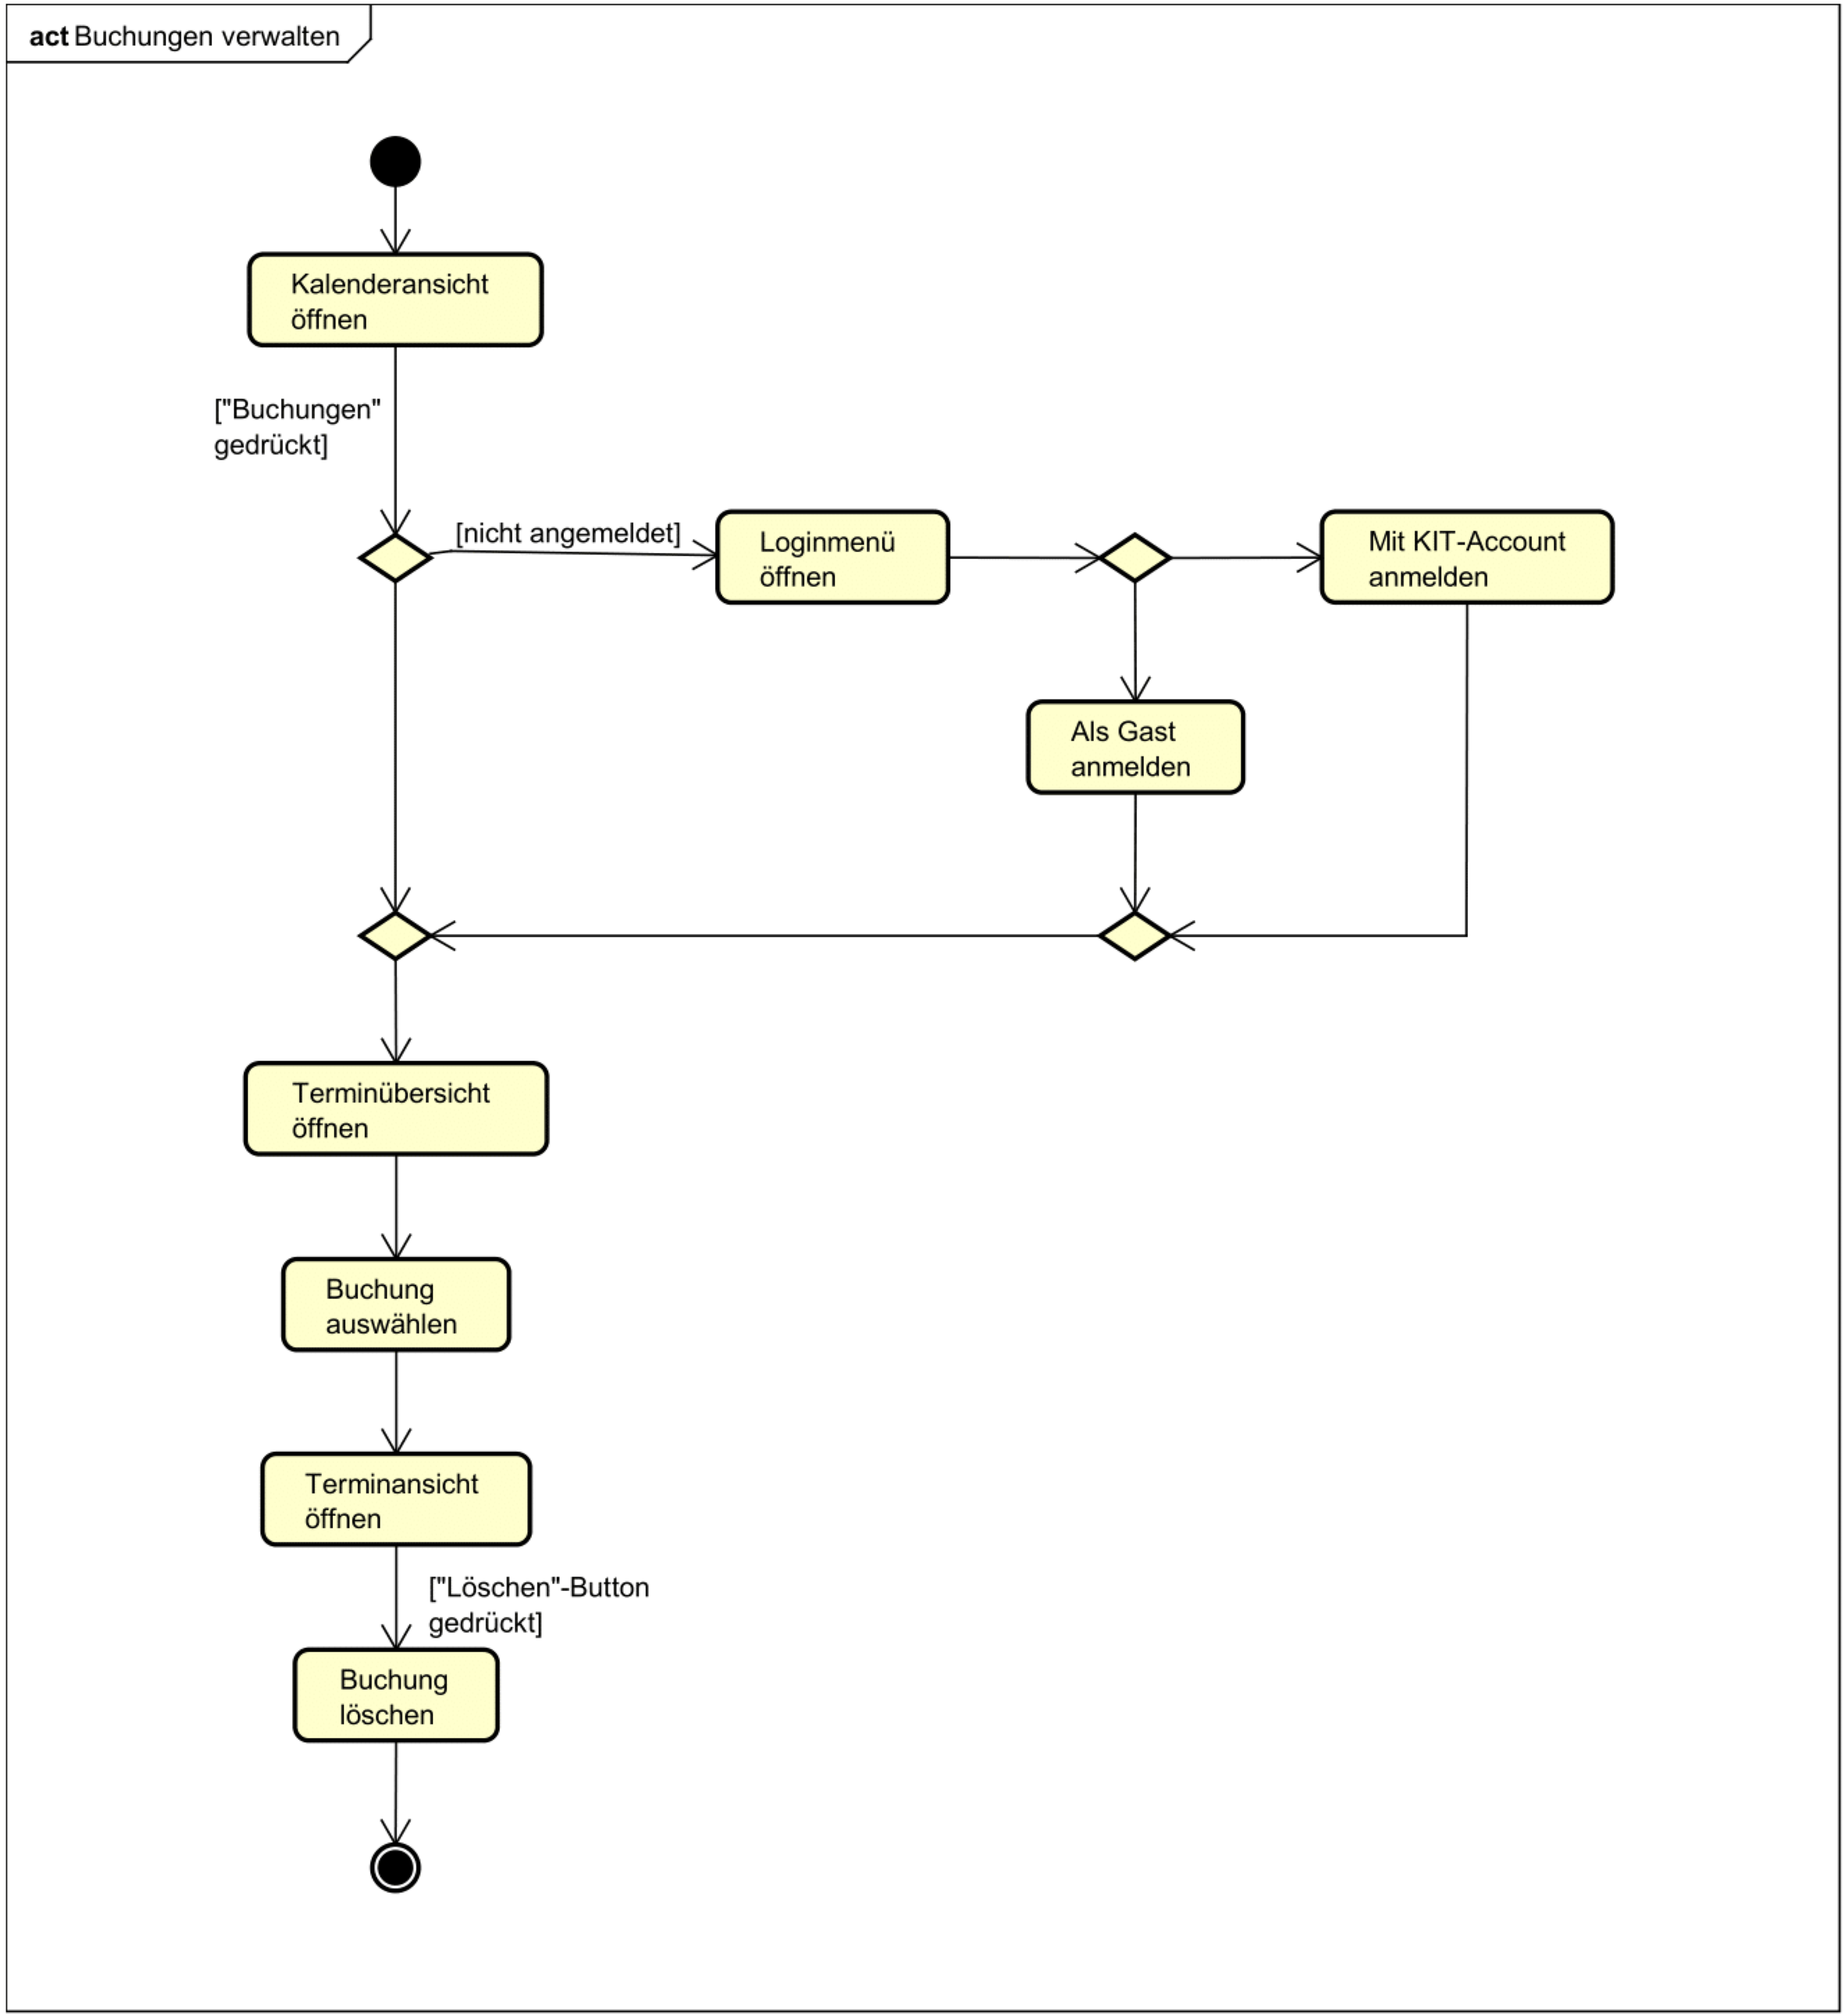
\includegraphics[width=\textwidth]{figures/activity/buchungverwalten}
    \caption{Diagramm zur Erklärung des Buchungsverwaltungsprozesses}
    \label{fig:manage-booking-diagram}
\end{figure}
\clearpage

\section{Terminaktionen}

Hier wird die Funktionalität der Terminansicht dargestellt. Wenn der angesehene Termin ein eigener Termin ist
oder man als Admin eingeloggt ist, gibt es hier die Möglichkeit den gewählten Termin zu löschen. Ist der
Termin nicht der eigene und er steht auf "auf Anfrage" teilen, dann gibt es einen Anfrage-Button über diesen man
eine Anfrage schicken kann.

\begin{figure}[ht]
    \centering
    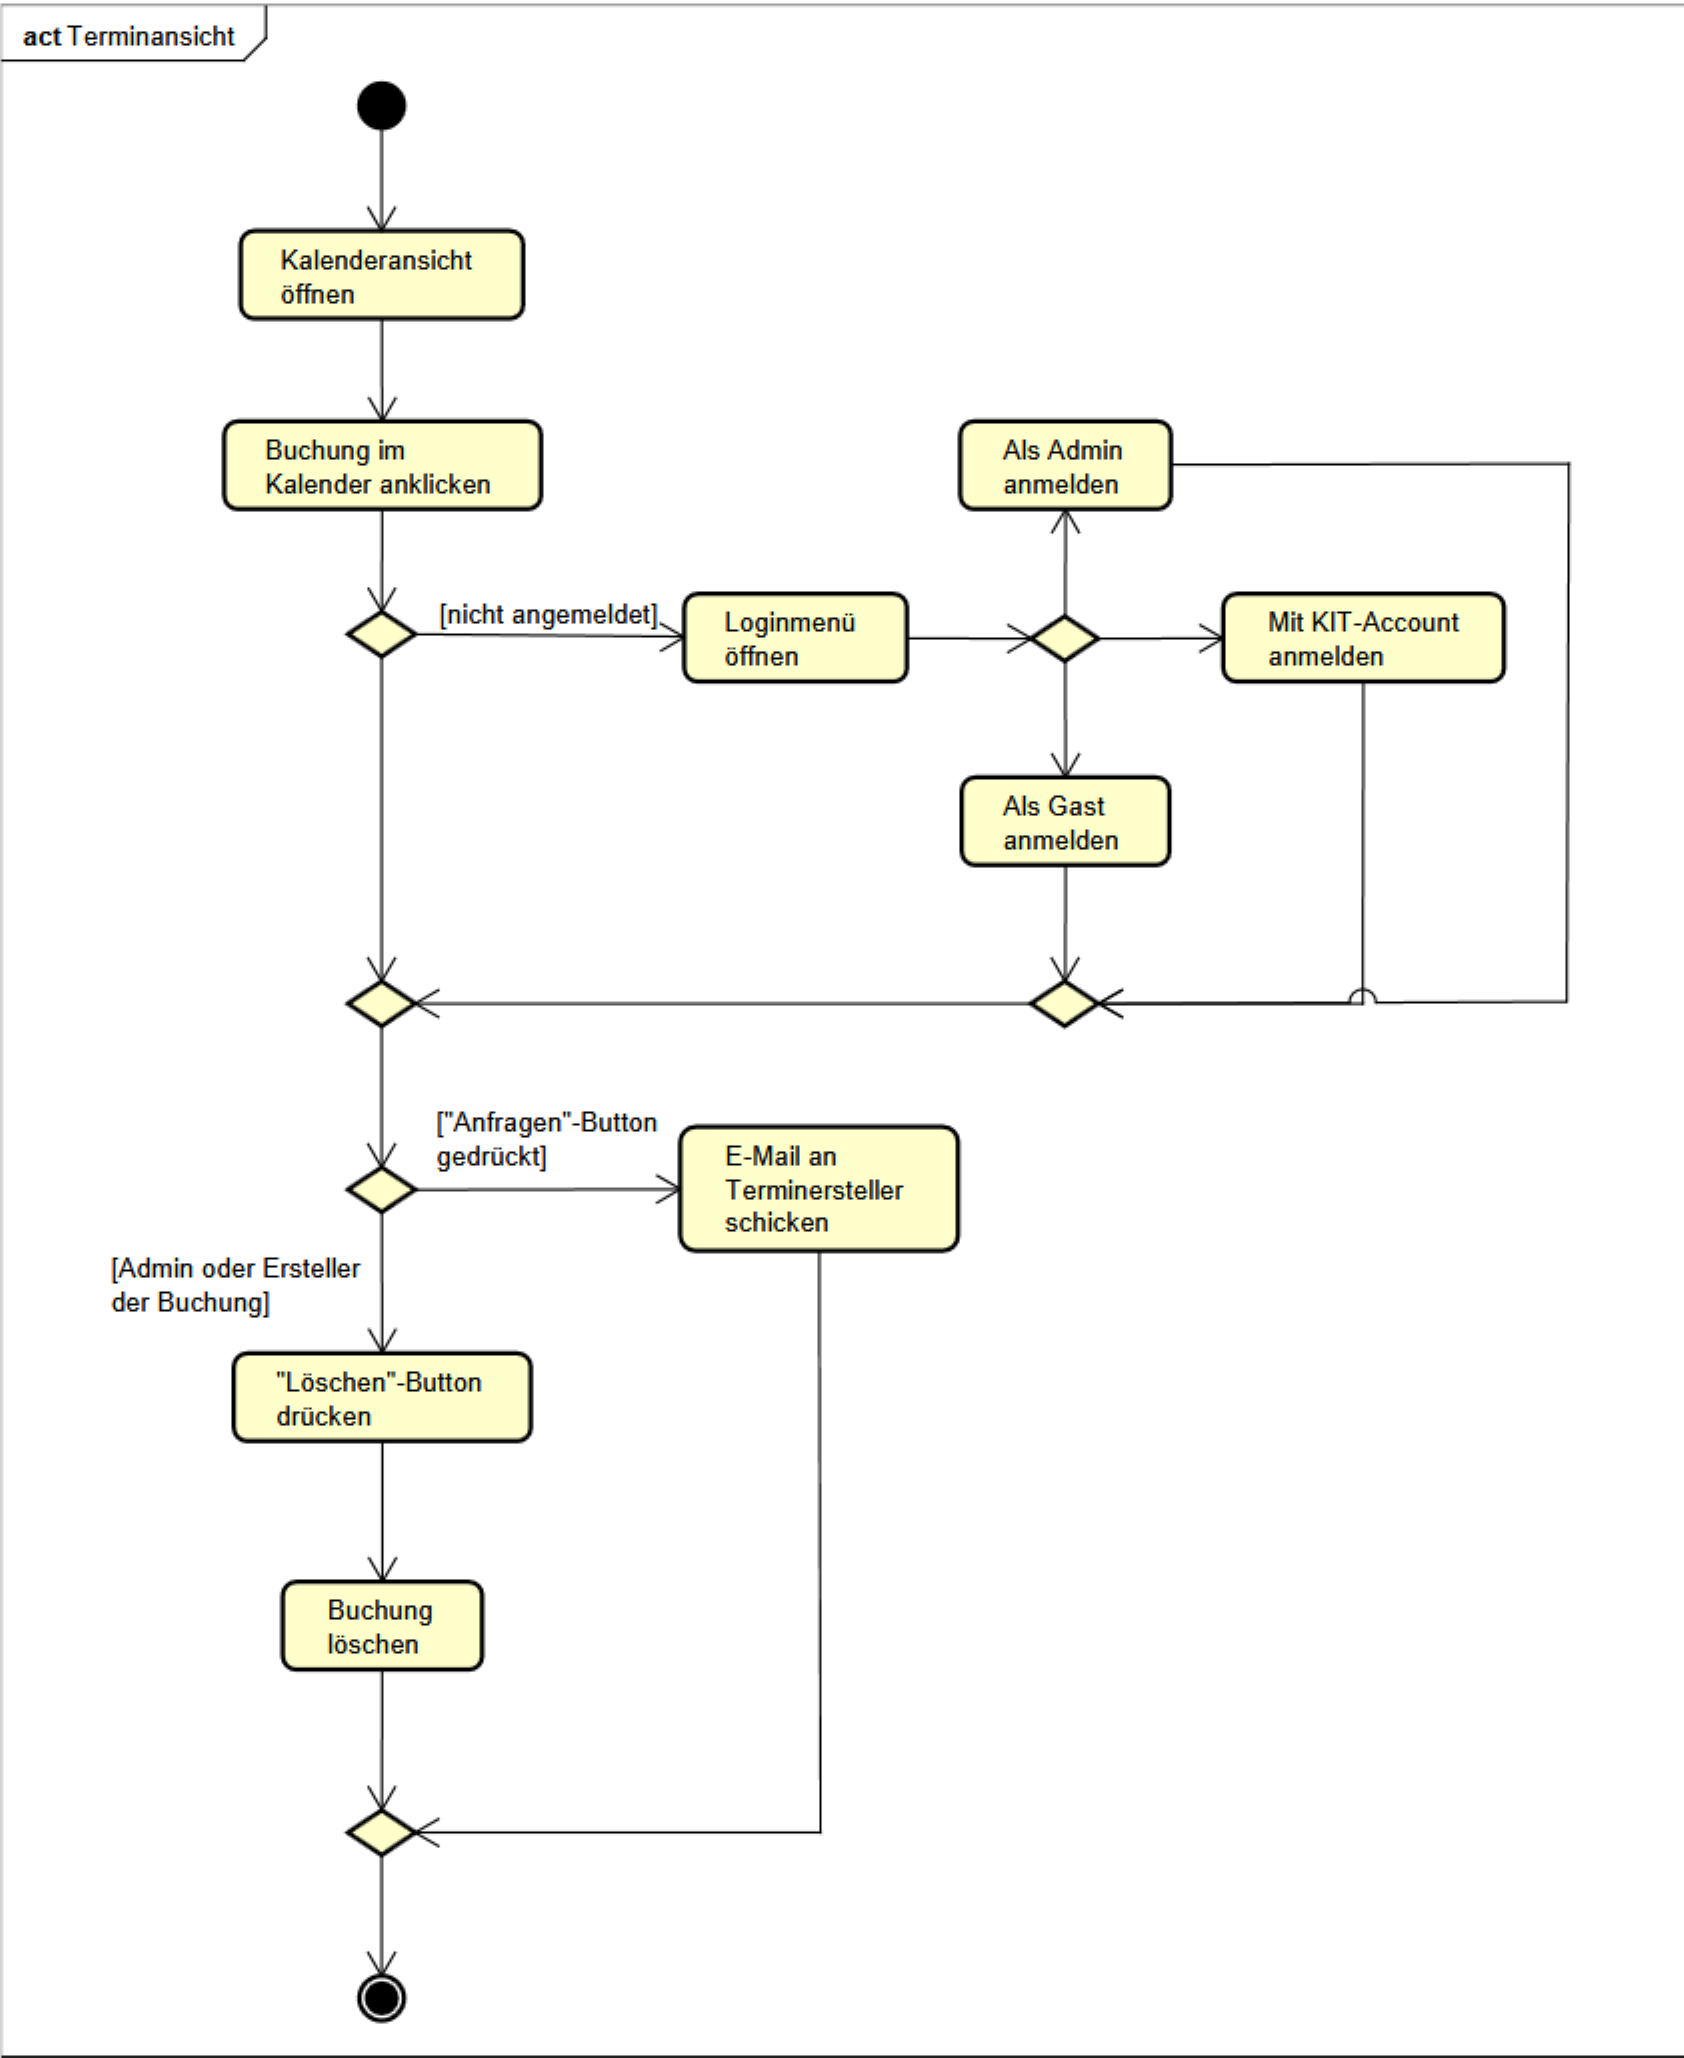
\includegraphics[width=\textwidth]{figures/activity/terminansicht}
    \caption{Diagramm zur Erklärung der Terminaktionen}
    \label{fig:booking-actions-diagram}
\end{figure}
\clearpage

\section{Abmeldeprozess}

Um sich von der Website abzumelden, gibt es einen Abmelde-Button.

Dieses Ablaufdiagramm beschreibt den Abmelde-Prozess.

\begin{figure}[ht]
    \centering
    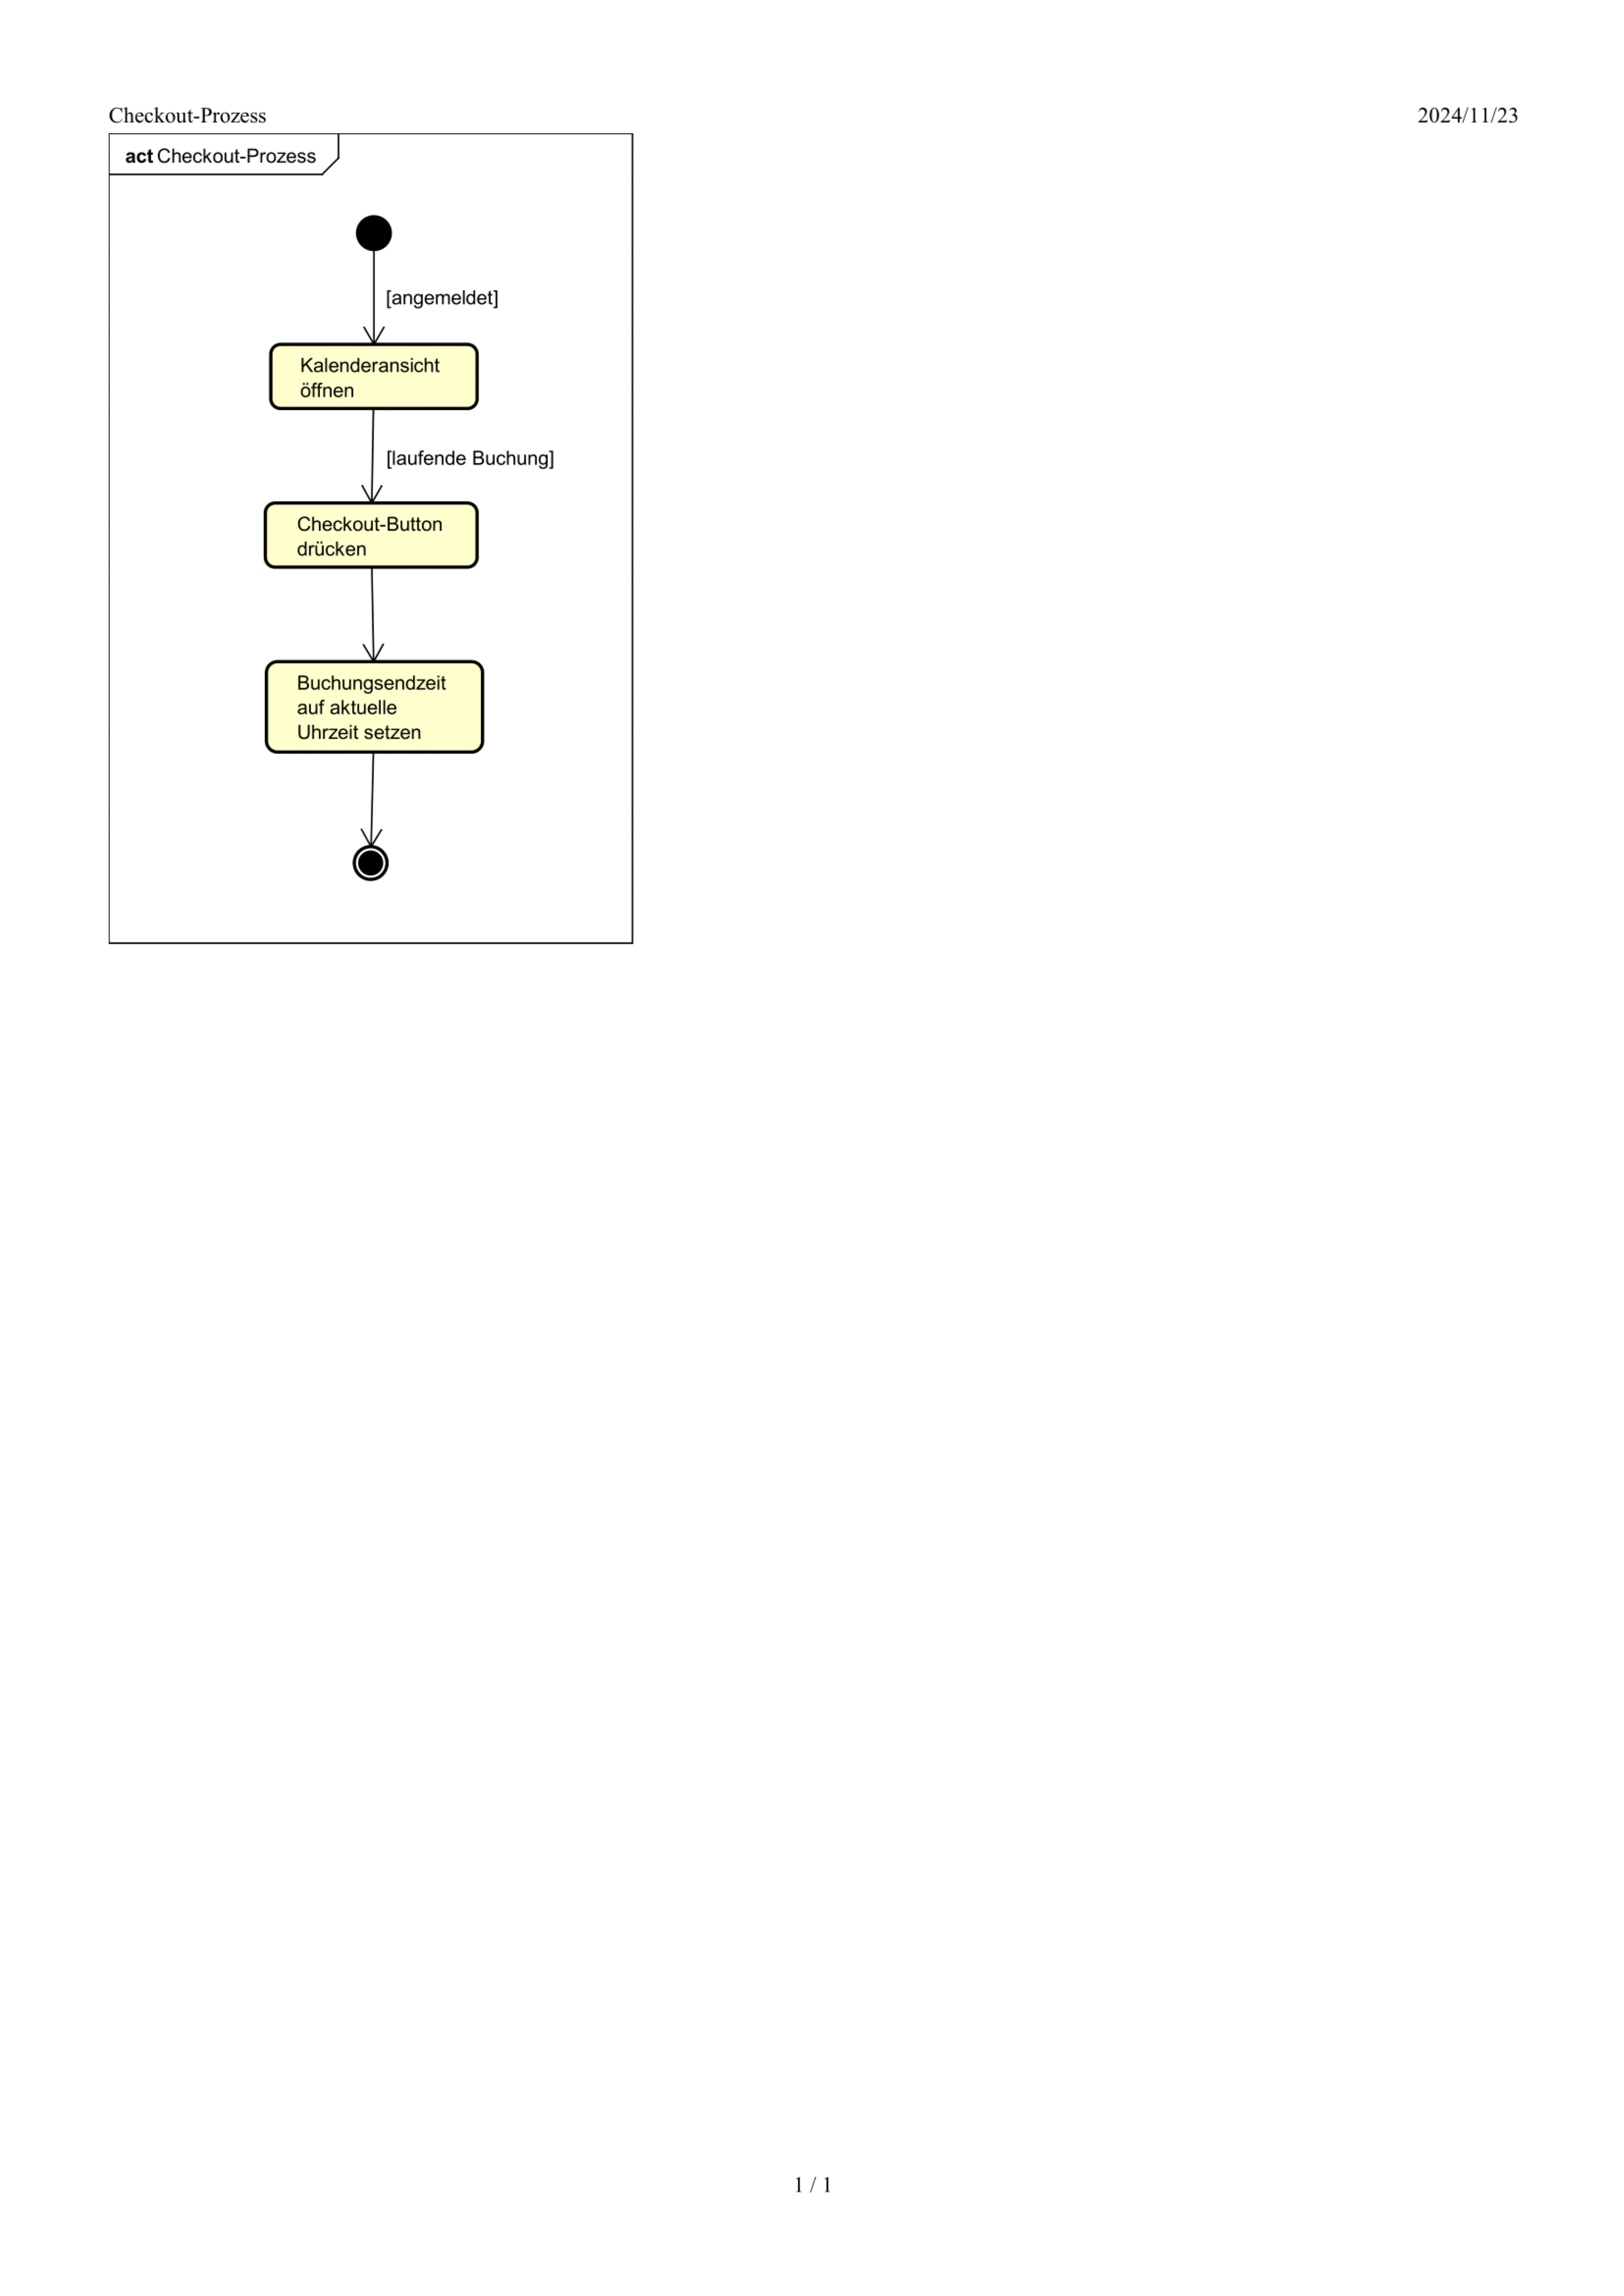
\includegraphics[width=\textwidth]{figures/activity/checkoutprozess}
    \caption{Diagramm zur Erklärung des Abmeldeprozesses}
    \label{fig:logout-diagram}
\end{figure}
\clearpage

\section{Adminfunktionalität}

Die Adminfunktionalität beinhaltet mehrere Möglichkeiten, die Website zu verwalten.
Es kann ein Termin gelöscht, Kontos gebannt, die Öffnungszeiten geändert und die Gästefunktion
ausgeschalten werden.

Dieses Ablaufdiagramm stellt die unterschiedlichen Aktionsmöglichkeiten des/r Admins dar.

\begin{figure}[ht]
    \centering
    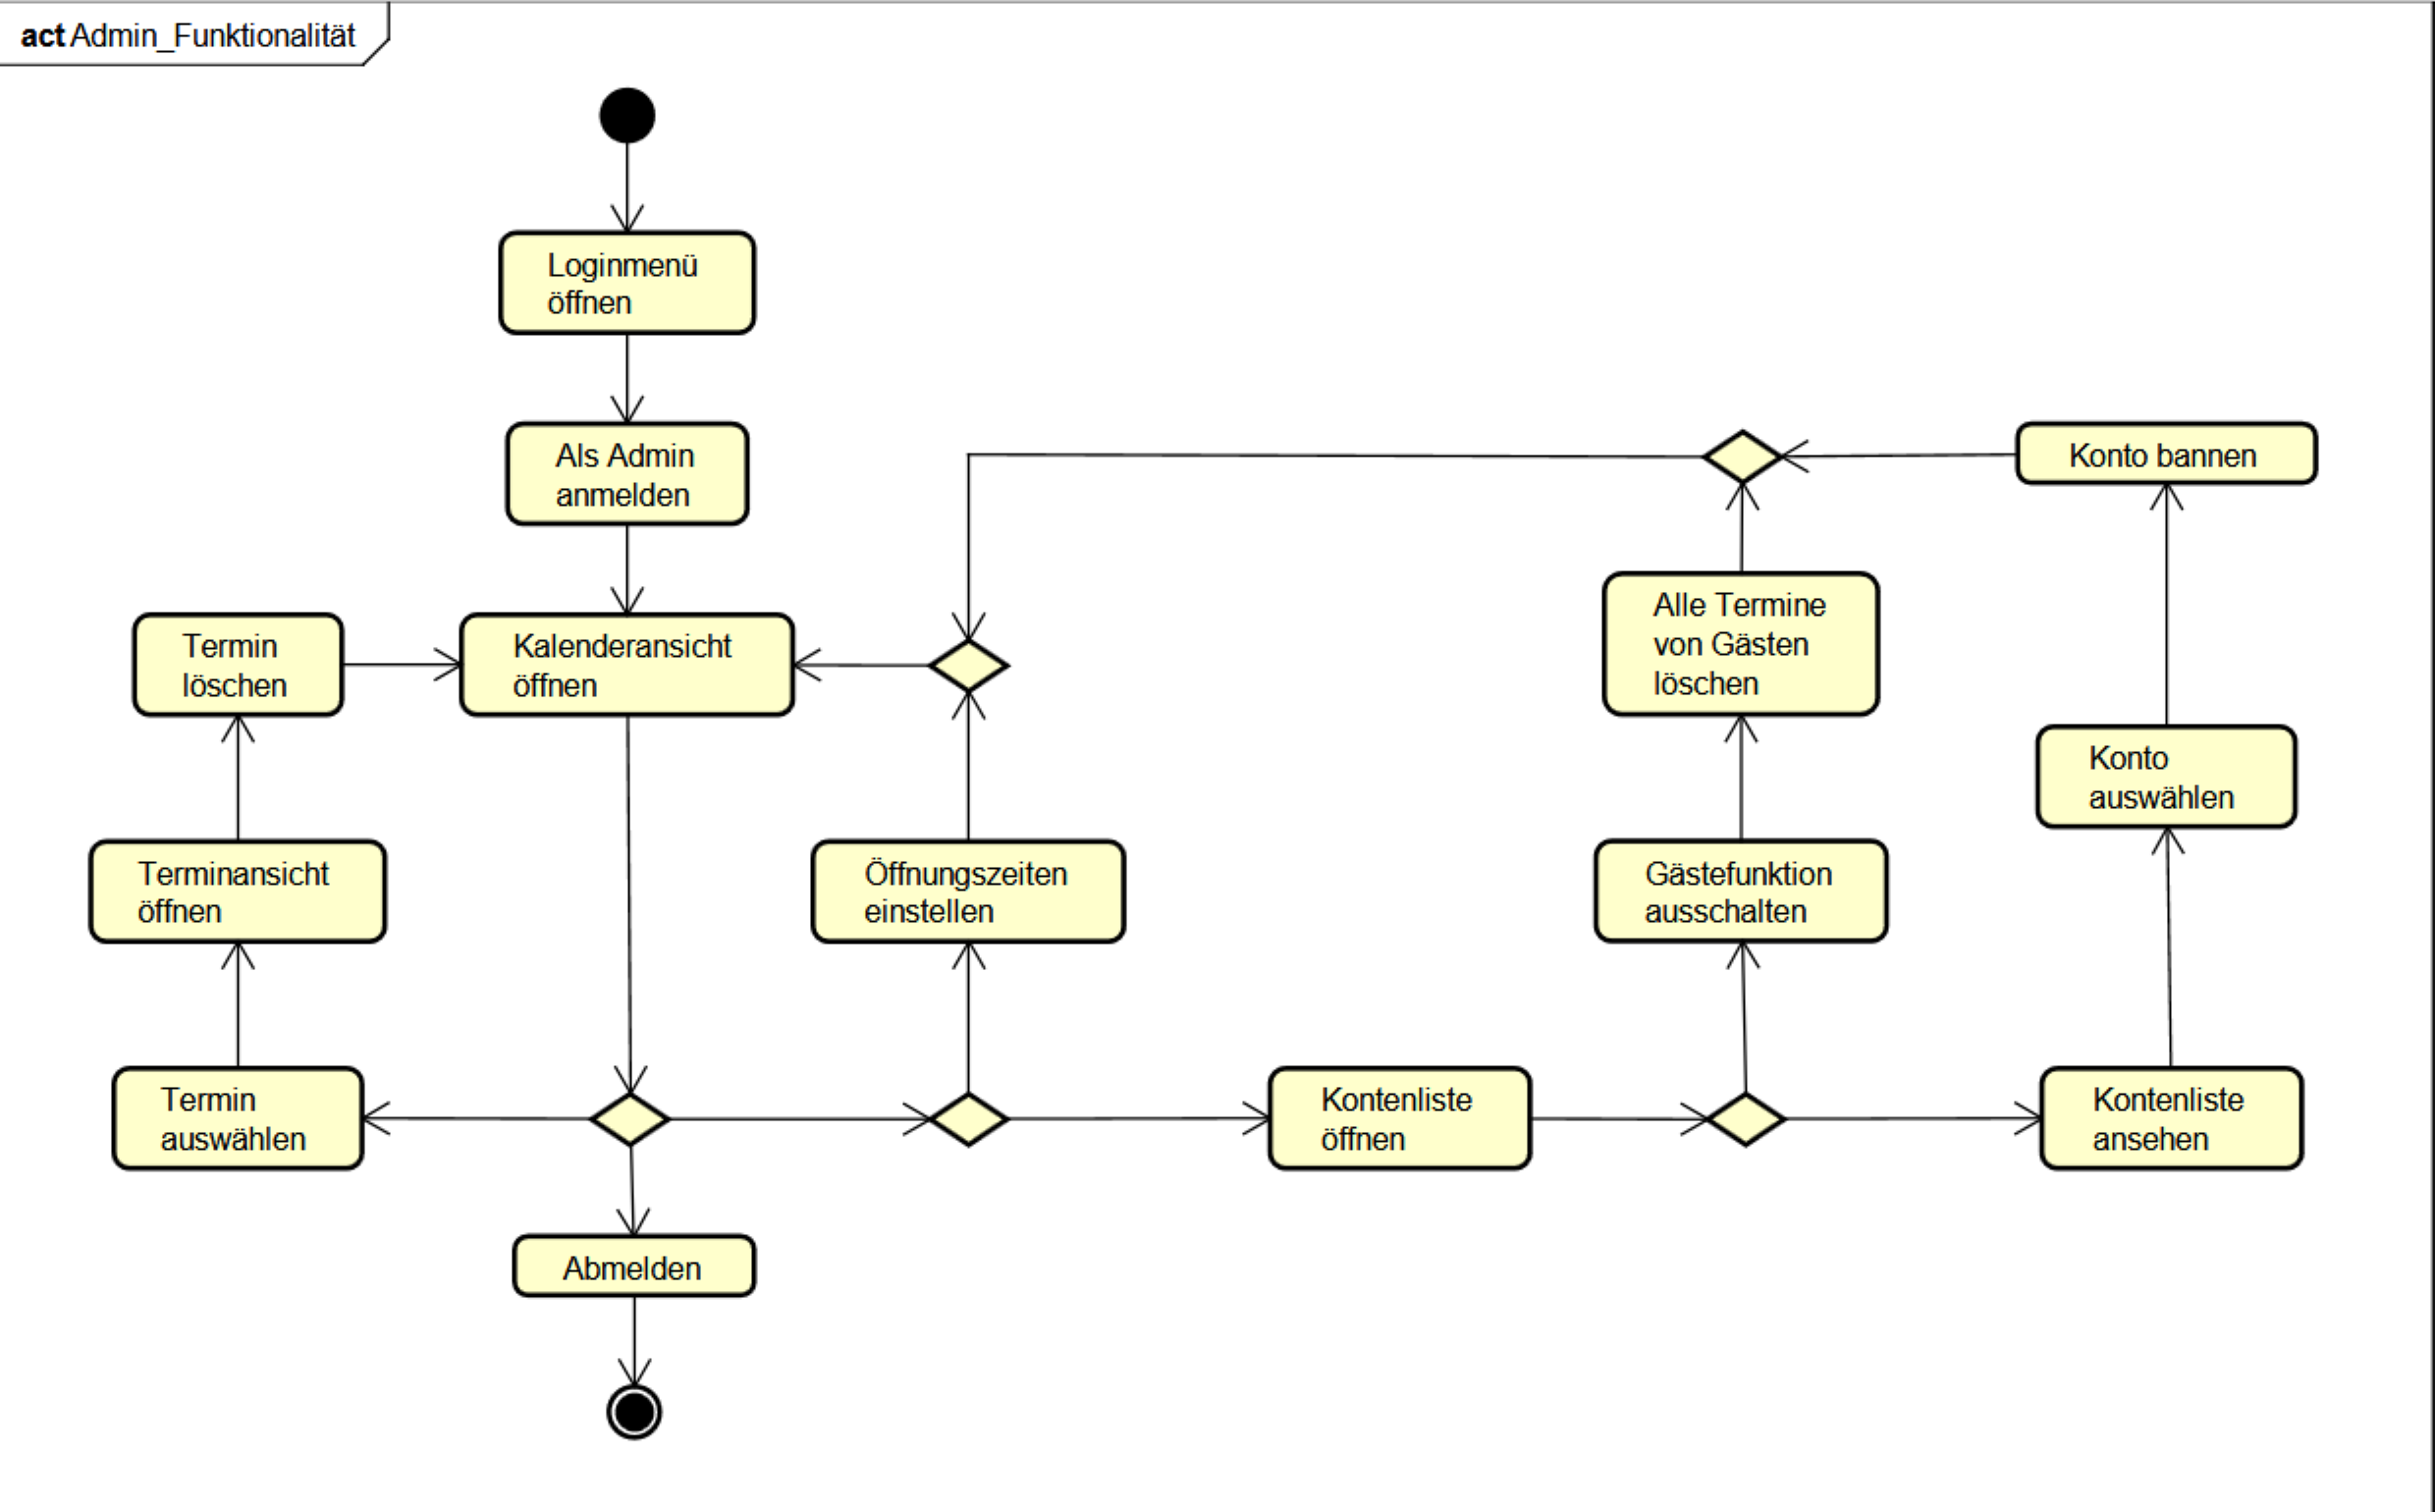
\includegraphics[width=\textwidth]{figures/activity/adminfunk}
    \caption{Diagramm zur Erklärung der Adminfunktionalität}
    \label{fig:admin-functions-diagram}
\end{figure}
\clearpage
